\documentclass[10.5pt,letterpaper]{article}
\usepackage{graphicx}
\usepackage{scrextend}
\usepackage{vmargin}
\usepackage[utf8]{inputenc}
\usepackage[spanish]{babel}
\usepackage{multicol}
\usepackage{amsmath, amsthm, amssymb, amsfonts}
\usepackage[usenames]{color}
\parindent=0mm
\pagestyle{empty}
\definecolor{miorange}{rgb}{0.91, 0.43, 0.0}
\begin{document}
\setmargins{2.5cm}      
{1.5cm}                     
{2cm}  
{24cm}                    
{10pt}                          
{1cm}                          
{0pt}                             
{2cm}
\begin{flushleft}
Examen Prueba
\end{flushleft}
\vspace{-1.1cm}
\begin{flushright}
\today
\end{flushright}
\begin{multicols}{2}
\begin{enumerate}
\item El compuesto que se usa para cultivar orquídeas se prepara con 3 kilogramos de musgo por cada 5 kilogramos de cáscara de pino. Si se van a preparar 12 kilogramos del compuesto, ¿cuántos kilogramos de cáscara de pino se necesitan?\\

\begin{minipage}{0.23\linewidth}
\begin{enumerate}
\item[a)] 5
\end{enumerate}
\end{minipage}
\begin{minipage}{0.23\linewidth}
\begin{enumerate}
\item[b)] $\frac{96}{5}$
\end{enumerate}
\end{minipage}
\begin{minipage}{0.23\linewidth}
\begin{enumerate}
\item[c)] $\frac{15}{2}$
\end{enumerate}
\end{minipage}
\begin{minipage}{0.22\linewidth}
\begin{enumerate}
\item[d)] 8
\end{enumerate}
\end{minipage}
\item ¿Cuántos números diferentes hay de cuatro dígitos, en los que cada dígito sea mayor a 5?\\

\begin{minipage}{0.24\linewidth}
\begin{enumerate}
\item[a)] 100
\end{enumerate}
\end{minipage}
\begin{minipage}{0.24\linewidth}
\begin{enumerate}
\item[b)] 120
\end{enumerate}
\end{minipage}
\begin{minipage}{0.24\linewidth}
\begin{enumerate}
\item[c)] 625
\end{enumerate}
\end{minipage}
\begin{minipage}{0.24\linewidth}
\begin{enumerate}
\item[d)] 256
\end{enumerate}
\end{minipage}
\item Si $2A+b=5$, entonces $4a+2b=$\\

\begin{minipage}{0.24\linewidth}
\begin{enumerate}
\item[a)] 1
\end{enumerate}
\end{minipage}
\begin{minipage}{0.24\linewidth}
\begin{enumerate}
\item[b)] 10
\end{enumerate}
\end{minipage}
\begin{minipage}{0.24\linewidth}
\begin{enumerate}
\item[c)] 2.5
\end{enumerate}
\end{minipage}
\begin{minipage}{0.24\linewidth}
\begin{enumerate}
\item[d)] 20
\end{enumerate}
\end{minipage}
\item Si el 90 por ciento de P es igual al 30 por ciento de Q, ¿qué por ciento de P es Q?\\

\begin{minipage}{0.24\linewidth}
\begin{enumerate}
\item[a)] 3
\end{enumerate}
\end{minipage}
\begin{minipage}{0.24\linewidth}
\begin{enumerate}
\item[b)] 270
\end{enumerate}
\end{minipage}
\begin{minipage}{0.24\linewidth}
\begin{enumerate}
\item[c)] 30
\end{enumerate}
\end{minipage}
\begin{minipage}{0.24\linewidth}
\begin{enumerate}
\item[d)] 300
\end{enumerate}
\end{minipage}
\item Un número es divisible por 9 si la suma de sus dígitos es divisible por 9. ¿Cuál de los siguientes
números es divisible por 45?\\ 

\begin{minipage}{0.28\linewidth}
\begin{enumerate}
\item[a)] 63435
\end{enumerate}
\end{minipage}
\begin{minipage}{0.28\linewidth}
\begin{enumerate}
\item[b)] 72365
\end{enumerate}
\end{minipage}\\
\begin{minipage}{0.28\linewidth}
\begin{enumerate}
\item[c)] 99999
\end{enumerate}
\end{minipage}
\begin{minipage}{0.28\linewidth}
\begin{enumerate}
\item[d)] 98145
\end{enumerate}
\end{minipage}
\item El costo de dos joyas iguales, con el impuesto incluido, es \$30.80. El impuesto por cada joya es \$1.27. ¿Cuál es el precio de una sola joya sin incluir el impuesto?\\

\begin{minipage}{0.3\linewidth}
\begin{enumerate}
\item[a)] \$14.13
\end{enumerate}
\end{minipage}
\begin{minipage}{0.3\linewidth}
\begin{enumerate}
\item[b)] \$28.56
\end{enumerate}
\end{minipage}\\
\begin{minipage}{0.3\linewidth}
\begin{enumerate}
\item[c)] \$15.40
\end{enumerate}
\end{minipage}
\begin{minipage}{0.3\linewidth}
\begin{enumerate}
\item[d)] \$29.53
\end{enumerate}
\end{minipage}
\item Si $4^n \times 8^n = 2^{10}$, entonces n=\\
\begin{minipage}{0.23\linewidth}
\begin{enumerate}
\item[a)] 8
\end{enumerate}
\end{minipage}
\begin{minipage}{0.23\linewidth}
\begin{enumerate}
\item[b)] 2
\end{enumerate}
\end{minipage}
\begin{minipage}{0.23\linewidth}
\begin{enumerate}
\item[c)] 5
\end{enumerate}
\end{minipage}
\begin{minipage}{0.23\linewidth}
\begin{enumerate}
\item[d)] 6
\end{enumerate}
\end{minipage}
\item La pendiente de la recta con ecuación \\$9x–3y=12$ es\\
\begin{minipage}{0.23\linewidth}
\begin{enumerate}
\item[a)] 9
\end{enumerate}
\end{minipage}
\begin{minipage}{0.23\linewidth}
\begin{enumerate}
\item[b)] 3
\end{enumerate}
\end{minipage}
\begin{minipage}{0.23\linewidth}
\begin{enumerate}
\item[c)] 4
\end{enumerate}
\end{minipage}
\begin{minipage}{0.23\linewidth}
\begin{enumerate}
\item[d)] 12
\end{enumerate}
\end{minipage}
\item En la siguiente figura, el área sombreada es igual a 3$u^2$, ¿cuantas $u^2$ en el área del cuadrado?
\begin{center}
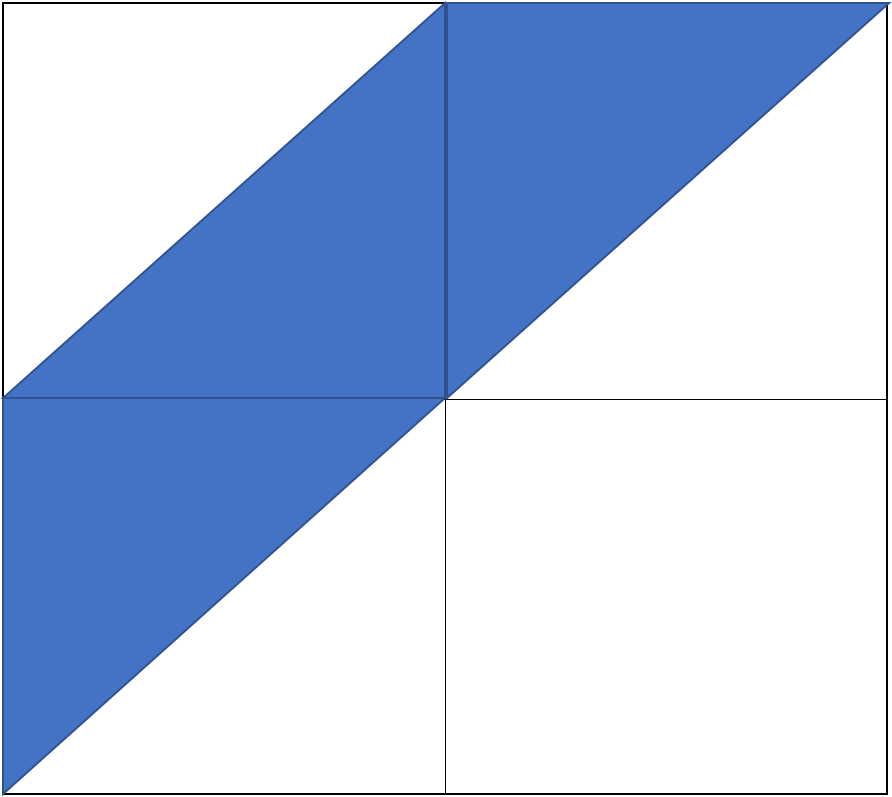
\includegraphics[scale=0.2]{images/f1.png}
\end{center}
\begin{minipage}{0.23\linewidth}
\begin{enumerate}
\item[a)] 1
\end{enumerate}
\end{minipage}
\begin{minipage}{0.23\linewidth}
\begin{enumerate}
\item[b)] 5
\end{enumerate}
\end{minipage}
\begin{minipage}{0.23\linewidth}
\begin{enumerate}
\item[c)] 6
\end{enumerate}
\end{minipage}
\begin{minipage}{0.23\linewidth}
\begin{enumerate}
\item[d)] 8
\end{enumerate}
\end{minipage}
\item ¿Cual es la suma de las medidas de los ángulos señalados?
\begin{center}
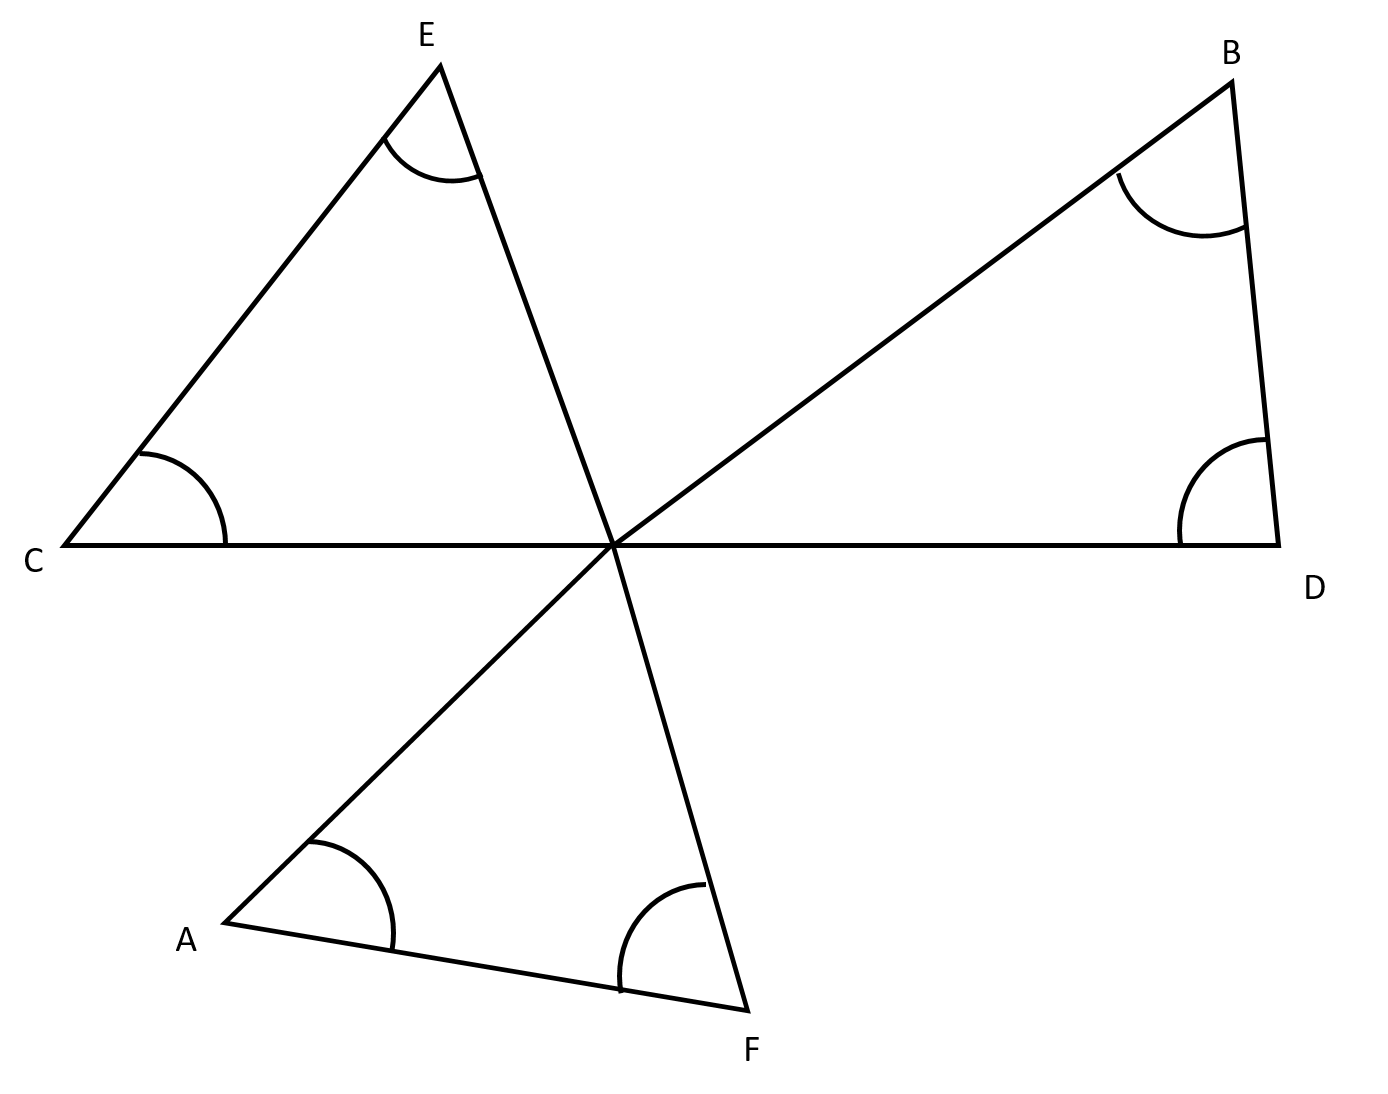
\includegraphics[scale=0.2]{images/F2.png}
\end{center}
\begin{minipage}{0.23\linewidth}
\begin{enumerate}
\item[a)] 180
\end{enumerate}
\end{minipage}
\begin{minipage}{0.23\linewidth}
\begin{enumerate}
\item[b)] 270
\end{enumerate}
\end{minipage}
\begin{minipage}{0.23\linewidth}
\begin{enumerate}
\item[c)] 360
\end{enumerate}
\end{minipage}
\begin{minipage}{0.23\linewidth}
\begin{enumerate}
\item[d)] 720
\end{enumerate}
\end{minipage}
\item El costo de dos joyas iguales, con el impuesto incluido, es \$30.90. El impuesto por cada joya es \$1.27. ¿Cuál es el precio de una sola joya sin incluir el impuesto?
\begin{minipage}{0.23\linewidth}
\begin{enumerate}
\item[a)] 29.53
\end{enumerate}
\end{minipage}
\begin{minipage}{0.23\linewidth}
\begin{enumerate}
\item[b)] 14.13
\end{enumerate}
\end{minipage}
\begin{minipage}{0.23\linewidth}
\begin{enumerate}
\item[c)] 14.76
\end{enumerate}
\end{minipage}
\begin{minipage}{0.23\linewidth}
\begin{enumerate}
\item[d)] 28.26
\end{enumerate}
\end{minipage}
\item Los calcetines se venden a  \$1 el par o a 2 por \$1.99. Si José compra 2 pares, ¿qué por ciento del costo total se ahorra, a razón del precio de un solo par?
\begin{minipage}{0.23\linewidth}
\begin{enumerate}
\item[a)] 10\%
\end{enumerate}
\end{minipage}
\begin{minipage}{0.23\linewidth}
\begin{enumerate}
\item[b)] 0.5\%
\end{enumerate}
\end{minipage}
\begin{minipage}{0.23\linewidth}
\begin{enumerate}
\item[c)] 5\%
\end{enumerate}
\end{minipage}
\begin{minipage}{0.23\linewidth}
\begin{enumerate}
\item[d)] 1\%
\end{enumerate}
\end{minipage}
\item En un aula, la asignatura de gimnasia la han aprobado el 62,5\% de las alumnas y el 80\% de los alumnos, mientras que la asignatura de historia la han aprobado 87,5\% de las alumnas y el 60\% de los alumnos:
\begin{center}
\begin{tabular}{|c|c|c|}
\hline
& Gimnasia & Historia \\ \hline
Alumnas & 62.5\% & 87.5\% \\ \hline
Alumnos & 80\% & 60\% \\ \hline
Total & 26 & 26 \\ \hline
\end{tabular}
\end{center}
Calcular el número de alumnas y de alumnos que hay en el aula si el total de aprobados es 26 en gimnasia y 26 en historia.
\item Hallar un número de tres cifras sabiendo que la suma de sus cifras es 11, que la suma de la primera y la tercera cifra es 5 y que la segunda cifra es el doble de la tercera.
\item Si $2x+3=-4$, entonces ¿cuál es el valor de $(2x+3)^2+3(2x+3)-4$\\
\begin{minipage}{0.23\linewidth}
\begin{enumerate}
\item[a)] 0
\end{enumerate}
\end{minipage}
\begin{minipage}{0.23\linewidth}
\begin{enumerate}
\item[b)] 4
\end{enumerate}
\end{minipage}
\begin{minipage}{0.23\linewidth}
\begin{enumerate}
\item[c)] -4
\end{enumerate}
\end{minipage}
\begin{minipage}{0.23\linewidth}
\begin{enumerate}
\item[d)] 12
\end{enumerate}
\end{minipage}
\item Si p es mayor que 3 y p es un factor de 18, de 24 y de 36, ¿cuál de los siguientes números es un posible valor de p?\\
\begin{minipage}{0.23\linewidth}
\begin{enumerate}
\item[a)] 6
\end{enumerate}
\end{minipage}
\begin{minipage}{0.23\linewidth}
\begin{enumerate}
\item[b)] 9
\end{enumerate}
\end{minipage}
\begin{minipage}{0.23\linewidth}
\begin{enumerate}
\item[c)] 12
\end{enumerate}
\end{minipage}
\begin{minipage}{0.23\linewidth}
\begin{enumerate}
\item[d)] 18
\end{enumerate}
\end{minipage}
\item La proyección del volumen de ventas de juegos de videos está dada por la relación:
\begin{equation*}
s(p)=\frac{3000}{2p+q}
\end{equation*}
donde s es el número de juegos vendidos en miles, p es el precio de un juego, en dolares, y q es una constante. Si, de acuerdo con la proyección, se venden 100,000 juegos a \$10 por juego. ¿cuantos juegos se venderan a \$20 por juego?\\
\begin{minipage}{0.34\linewidth}
\begin{enumerate}
\item[a)] 50,000
\end{enumerate}
\end{minipage}
\begin{minipage}{0.34\linewidth}
\begin{enumerate}
\item[b)] 60,000
\end{enumerate}
\end{minipage}\\
\begin{minipage}{0.34\linewidth}
\begin{enumerate}
\item[c)] 150,000
\end{enumerate}
\end{minipage}
\begin{minipage}{0.34\linewidth}
\begin{enumerate}
\item[d)]200,000
\end{enumerate}
\end{minipage}
\item Margarita hace flanes de calabaza para la venta. Ella no compra calabazas que pesen menos de 2 libras ni más de 10 libras. Si x representa el peso en libras de las calabazas que no compra Margarita. ¿cuál de las siguientes opciones representa todos los posibles valores de x?\\
\begin{minipage}{0.5\linewidth}
\begin{enumerate}
\item[a)] $|x-2|>10$
\end{enumerate}
\end{minipage}\\
\begin{minipage}{0.5\linewidth}
\begin{enumerate}
\item[b)] $|x-4|>6$
\end{enumerate}
\end{minipage}\\
\begin{minipage}{0.5\linewidth}
\begin{enumerate}
\item[c)] $|x-5|>5$
\end{enumerate}
\end{minipage}\\
\begin{minipage}{0.5\linewidth}
\begin{enumerate}
\item[d)]$|x-6|>4$
\end{enumerate}
\end{minipage}
\item ¿Para cuál valor de x es cierta la expresión $(x+1)^2=x^2+1$
\begin{enumerate}
\item Para todo valor de x
\item x=0, solamente
\item x=1, solamente
\item x=-1, solamente
\end{enumerate}
\item Las temperaturas durante la semana en una ciudad son las siguientes:
\begin{center}
\begin{tabular}{|c|c|}
\hline
Dia & Temperatura\\ \hline
Lunes & 66\\ \hline
Martes & 78\\ \hline
Miércoles & 75\\ \hline
Jueves & 69\\ \hline
Viernes & 78\\ \hline
Sábado & 77\\ \hline
Domingo & 70\\ \hline
\end{tabular}
\end{center}
si P representa la mediana, q la moda y r el promedio. ¿cuál de las siguientes opciones presenta el orden correcto de p,q,r?
\begin{enumerate}
\item $r<p<q$
\item $r<q<p$
\item $p<r<q$
\item $p=q=r$
\end{enumerate}
\item Tres cajas contienen, cada una, 12 kilogramos de carne de res, 18 de carne de cerdo y 24 de carne de pollo. La carne de cada caja está contenida en bolsas del mismo tamaño y con la máxima cantidad de carne posible, ¿cuánto pesa cada bolsa y cuántas hay por caja?
\item Un grupo de 45 estudiantes de CONAMAT contrata un autobús para ir a un evento y calculan que cada uno debe pagar
\$50; finalmente sólo asisten 30 estudiantes, ¿cuánto deberá pagar cada uno?
\item Simplifica la siguiente expresión:
\begin{equation*}
\frac{5}{2}x^2-5xy+\frac{2}{3}y^2+\left(-\frac{1}{3}x^2+\frac{3}{2}xy-\frac{1}{4}y^2 \right)
\end{equation*}
\item Se ordenan en una fila 5 bolas rojas, 2 bolas blancas y 3 bolas azules.
Si las bolas de igual color no se distinguen entre sí.
¿De cuántas formas posibles pueden ordenarse?
\item Una urna tiene ocho bolas rojas, 5 amarilla y siete verdes. Si se extrae una
bola al azar calcular la probabilidad de:
\begin{enumerate}
\item Sea roja.
\item  Sea verde.
\item  Sea amarilla.
\item  No sea roja.
\item  No sea amarilla.
\end{enumerate}
\item Un avión dispone de 32 asientos en clase A y de 50 asientos en clase B cuya venta supone un total de 14.600. Sin embargo, sólo sea han vendido 10 asientos en clase A y 40 en clase B, obteniendo un total de 7.000. Calcule el costo de la clase A y B.
\item 11 obreros labran un campo rectangular de 220 m de largo y 48 de ancho en 6 días.
¿Cuántos obreros serán necesarios para labrar otro campo análogo de 300 m de
largo por 56 m de ancho en cinco días?
\item Resuleve la siguiente desigualdad cuadrática 
\begin{equation*}
x(3x+2)>(x+2)2
\end{equation*}
\item Con una cuerda de 34 metros se puede dibujar un rectángulo (sin que sobre cuerda) cuya diagonal mide 13 metros.
Calcular cuánto mide la base y la altura de dicho rectángulo.
\item Simplifica la siguiente expresión
\begin{equation*}
5\sqrt{8}-\sqrt{27}-\sqrt{32}+3\sqrt{3}+\sqrt{2}
\end{equation*}
\item Para aprobar un examen de 60 reactivos, Mónica tiene que contestar correctamente 75\% de éste, ¿cuál es el mínimo
de preguntas que deberá contestar acertadamente para aprobarlo?	
\item Dos ciudades M y N se encuentran a 640 km de distancia entre sí. A las 10 de la mañana de la ciudad M sale un
automóvil rumbo a la ciudad N, con una velocidad de 85
km/h, a la misma hora de N sale otro automóvil rumbo a M
con una velocidad de 75
km/h, ¿a qué hora se encontrarán y qué distancia ha recorrido cada uno?
\end{enumerate}
\end{multicols}
\end{document}